% 声明文档类型为 standalone,这样输出的 pdf/png 尺寸会正好包裹住图像
% 'border=8pt' 选项在图像周围留出8pt的白边
% 'multi, tikz' 允许多个 tikz picture 环境
\documentclass[border=8pt, multi, tikz]{standalone}

\usepackage{import}
\usepackage{pgfplots}
\pgfplotsset{compat=1.18}
\usepgfplotslibrary{fillbetween}
\subimport{./layers/}{init}
\usetikzlibrary{positioning,calc}
\usepackage{graphicx}
\usetikzlibrary{decorations.pathreplacing}
\usetikzlibrary{fit}
\usetikzlibrary{shadows.blur}
\usetikzlibrary{backgrounds} 

% 定义一系列颜色变量,用于不同类型的神经网络层,方便统一修改和管理
\def\FFCMColor{rgb,255:red,173;green,216;blue,230}      % 卷积层颜色 (用于 FFCM)
\def\BFCMColor{rgb,255:red,150;green,223;blue,150}      % 卷积层颜色 (用于 BFCM)
\def\ConvColor{rgb,255:red,156;green,201;blue,229}      % 卷积层颜色 (用于 1x1x1)
\def\ConvReluColor{rgb,255:red,179;green,205;blue,224}  % 卷积+激活层颜色
\def\PoolColor{rgb,255:red,255;green,255;blue,163}      % 池化层颜色
\def\UnpoolColor{rgb,255:red,211;green,211;blue,211}   % 上采样/反卷积层颜色
\def\CatColor{rgb,255:red,191;green,155;blue,219}       % 拼接层(Cnode)颜色
\def\SoftmaxColor{rgb,255:red,112;green,128;blue,144}   % Softmax/Sigmoid层颜色

% ====================================================================================
%                            在此处调整布局参数
% ====================================================================================
% 1. 宽度缩放系数
\def\EncoderWidthScale{1.5}      % 左侧编码器宽度系数
\def\BottleneckWidthScale{0.7}   % 中间瓶颈层宽度系数
\def\DecoderWidthScale{0.9}      % 右侧解码器宽度系数

% 2. 间距系数
\def\BlockSpacing{0.3}           % 调整这个值来控制所有模块之间的基础间距
% ====================================================================================

\begin{document}
\begin{tikzpicture}

% 定义一个名为 "cursor" 的坐标
\coordinate (cursor) at (0,0,0);

% --- 连接线和箭头的样式定义 ---
% 'connection' 用于网络主干路径的连接线
\tikzstyle{connection}=[ultra thick,every node/.style={sloped,allow upside down},draw=rgb:blue,4;red,1;green,4;black,3,opacity=0.7]
% 'copyconnection' 用于跳跃连接的线
\tikzstyle{copyconnection}=[ultra thick,every node/.style={sloped,allow upside down},draw={rgb:blue,4;red,1;green,1;black,3},opacity=0.7]

% 定义一个名为 framebox 的样式,用于绘制圆角虚线框
\tikzstyle{framebox} = [
    draw=gray,                  % 边框颜色
    rounded corners=15pt,       % <-- 在此调整圆角大小
    line width=1.2pt,           % <-- 在此调整线条粗细
    dash pattern=on 6pt off 4pt, % <-- 在此调整虚线间隔 (画6pt,空4pt)
    blur shadow={shadow blur steps=5} % 给边框加一点模糊阴影,让它更突出
]

% 定义两种在连接线中间使用的箭头
\newcommand{\copymidarrow}{\tikz \draw[-Stealth,line width =0.8mm,draw={rgb:blue,4;red,1;green,1;black,3}] (-0.3,0) -- ++(0.3,0);}

%%%%%%%%%%%%%%%%%%%%%%%%%%%%%%%%%%%%%%%%%%%%%%%%%%%%%%%%%%%%%%%%%%%%%%%%%%%%%%%%%%%%%%%%
%% 1. 编码器 (Encoder) - 左侧
%%%%%%%%%%%%%%%%%%%%%%%%%%%%%%%%%%%%%%%%%%%%%%%%%%%%%%%%%%%%%%%%%%%%%%%%%%%%%%%%%%%%%%%%
% --- FFCM1 ---
\def\BlockHeight{40} 
\pic at ($(cursor) + (0, \BlockHeight*0.1, 0)$) {RightBandedBox={name=FFCM1,
        xlabel={{"8",""}},ylabel=256x256,labelpos=0.92,labelyshift=-12pt,
        fill=\FFCMColor,bandfill=\ConvReluColor,
        height=\BlockHeight,width={\EncoderWidthScale*4,0},depth=\BlockHeight}};

%\coordinate (input_center) at ($(FFCM1-anchor) + (0, -10)$);
\coordinate (input_center) at ($(FFCM1-anchor) + (2.5cm, 10)$);
\coordinate (image_input_center) at ($(input_center) + (-1.1cm, 0)$);

\node[anchor=east] (img2) at ($(image_input_center) - (0.1cm,0)$)
    {
\includegraphics[width=1.6cm]{pic/图片1.png}};
\node[anchor=west] (ellipsis) at ($(image_input_center) + (0.1cm,0)$)
    {\Huge $\dots$};
\node[left=0.2cm of img2] (img1)
    {
\includegraphics[width=1.6cm]{pic/图片2.png}};
\node[right=0.2cm of ellipsis] (img3)
    {
\includegraphics[width=1.6cm]{pic/图片3.png}};
    
\draw [decorate, decoration={brace, amplitude=8pt, raise=4pt}, ultra thick, draw=\edgecolor]
    (img1.north west) -- (img3.north east)
    node[midway, above=12pt] (input_brace_label) {\Large\bfseries\itshape Input: D=5};
    
\coordinate (arrow_start_point) at ($(input_center |- img1.south) + (0, -0.1cm) + (-3.1cm, 0cm)$);
\coordinate (arrow_end_point) at ($(FFCM1-north) + (0, 0.5cm) + (-0.6cm, 1cm)$);

\draw[-{Stealth[length=3mm, width=2mm]}, ultra thick, draw=\edgecolor]
    (arrow_start_point) -- (arrow_end_point)
    node[midway, left=2mm] {};

\path (FFCM1-southeast) coordinate (cursor);

% --- Pool1 ---
\def\BlockHeight{32}
\pic at ($(cursor) + (0, \BlockHeight*0.1, 0)$) {Box={name=Pool1,
        fill=\PoolColor,opacity=0.7,height=\BlockHeight,width=\EncoderWidthScale*1,depth=\BlockHeight}};
\path (Pool1-southeast) ++(\BlockSpacing*1.5,0,0) coordinate (cursor);

% --- FFCM2 ---
\def\BlockHeight{32}
\pic at ($(cursor) + (0, \BlockHeight*0.1, 0)$) {RightBandedBox={name=FFCM2,
        xlabel={{"16",""}},ylabel=128x128,labelpos=0.9,labelyshift=-12pt,
        fill=\FFCMColor,bandfill=\ConvReluColor,
        height=\BlockHeight,width={\EncoderWidthScale*6,0},depth=\BlockHeight}};
\path (FFCM2-southeast) coordinate (cursor);

% --- Pool2 ---
\def\BlockHeight{25}
\pic at ($(cursor) + (0, \BlockHeight*0.1, 0)$) {Box={name=Pool2,
        fill=\PoolColor,opacity=0.7,height=\BlockHeight,width=\EncoderWidthScale*1,depth=\BlockHeight}};
\path (Pool2-southeast) ++(\BlockSpacing*1.5,0,0) coordinate (cursor);

% --- FFCM3 ---
\def\BlockHeight{25}
\pic at ($(cursor) + (0, \BlockHeight*0.1, 0)$) {RightBandedBox={name=FFCM3,
        xlabel={{"32",""}},ylabel=64x64,labelpos=0.90,labelyshift=-12pt,
        fill=\FFCMColor,bandfill=\ConvReluColor,
        height=\BlockHeight,width={\EncoderWidthScale*8,0},depth=\BlockHeight}};
\path (FFCM3-southeast) coordinate (cursor);

% --- Pool3 ---
\def\BlockHeight{16}
\pic at ($(cursor) + (0, \BlockHeight*0.1, 0)$) {Box={name=Pool3,
        fill=\PoolColor,opacity=0.7,height=\BlockHeight,width=\EncoderWidthScale*1,depth=\BlockHeight}};
\path (Pool3-southeast) ++(\BlockSpacing*1.0,0,0) coordinate (cursor);

% --- FFCM4 ---
\def\BlockHeight{16}
\pic at ($(cursor) + (0, \BlockHeight*0.1, 0)$) {RightBandedBox={name=FFCM4,
        xlabel={{"64",""}},ylabel=32x32,labelpos=0.84,labelyshift=-12pt,
        fill=\FFCMColor,bandfill=\ConvReluColor,
        height=\BlockHeight,width={\EncoderWidthScale*10,0},depth=\BlockHeight}};
\path (FFCM4-southeast) coordinate (cursor);

% --- Pool4 ---
\def\BlockHeight{8}
\pic at ($(cursor) + (0, \BlockHeight*0.1, 0)$) {Box={name=Pool4,
        fill=\PoolColor,opacity=0.7,height=\BlockHeight,width=\EncoderWidthScale*1,depth=\BlockHeight}};
\path (Pool4-southeast) ++(\BlockSpacing*1.0,0,0) coordinate (cursor);

%%%%%%%%%%%%%%%%%%%%%%%%%%%%%%%%%%%%%%%%%%%%%%%%%%%%%%%%%%%%%%%%%%%%%%%%%%%%%%%%%%%%%%%%
%% 2. 瓶颈层 (Bottleneck)
%%%%%%%%%%%%%%%%%%%%%%%%%%%%%%%%%%%%%%%%%%%%%%%%%%%%%%%%%%%%%%%%%%%%%%%%%%%%%%%%%%%%%%%%%
\def\BlockHeight{8}
\pic at ($(cursor) + (0, \BlockHeight*0.1, 0)$) {RightBandedBox={name=FFCM5,
        xlabel={{"128",""}},ylabel=16x16,labelpos=0.7,labelyshift=-12pt,
        fill=\FFCMColor,bandfill=\ConvReluColor,
        height=\BlockHeight,width={\BottleneckWidthScale*12,0},depth=\BlockHeight}};
\path (FFCM5-southeast) ++(\BlockSpacing*2.5,0,0) coordinate (cursor);

%%%%%%%%%%%%%%%%%%%%%%%%%%%%%%%%%%%%%%%%%%%%%%%%%%%%%%%%%%%%%%%%%%%%%%%%%%%%%%%%%%%%%%%%
%% 3. 解码器 (Decoder) - 右侧
%%%%%%%%%%%%%%%%%%%%%%%%%%%%%%%%%%%%%%%%%%%%%%%%%%%%%%%%%%%%%%%%%%%%%%%%%%%%%%%%%%%%%%%%
% --- 解码器阶段 1 (恢复至 32x32) ---
\def\BlockHeight{16}
\pic at ($(cursor) + (0, \BlockHeight*0.1, 0)$) {Box={name=Upscale1,
        fill=\UnpoolColor,opacity=0.7,height=\BlockHeight,width=\DecoderWidthScale*2,depth=\BlockHeight}};
\path (Upscale1-southeast) coordinate (cursor);

\pic at ($(cursor) + (0, \BlockHeight*0.1, 0)$) {RightBandedBox={name=Cnode1,
        xlabel={{"192",""}},fill=\CatColor,bandfill=\CatColor,opacity=0.7,
        height=\BlockHeight,width=\DecoderWidthScale*8,depth=\BlockHeight}};
\path (Cnode1-southeast) coordinate (cursor);

\pic at ($(cursor) + (0, \BlockHeight*0.1, 0)$) {RightBandedBox={name=BFCM1,
        xlabel={{"64",""}},ylabel=32x32,labelpos=0.84,labelyshift=-12pt,
        fill=\BFCMColor,bandfill=\BFCMColor, % MODIFIED: Changed to BFCMColor
        height=\BlockHeight,width={\DecoderWidthScale*6,0},depth=\BlockHeight}};
\path (BFCM1-southeast) ++(\BlockSpacing*2.0,0,0) coordinate (cursor);

% --- 解码器阶段 2 (恢复至 64x64) ---
\def\BlockHeight{25}
\pic at ($(cursor) + (0, \BlockHeight*0.1, 0)$) {Box={name=Upscale2,
        fill=\UnpoolColor,opacity=0.7,height=\BlockHeight,width=\DecoderWidthScale*2,depth=\BlockHeight}};
\path (Upscale2-southeast) coordinate (cursor);

\pic at ($(cursor) + (0, \BlockHeight*0.1, 0)$) {RightBandedBox={name=Cnode2,
        xlabel={{"96",""}},fill=\CatColor,bandfill=\CatColor,opacity=0.7,
        height=\BlockHeight,width=\DecoderWidthScale*7,depth=\BlockHeight}};
\path (Cnode2-southeast) coordinate (cursor);

\pic at ($(cursor) + (0, \BlockHeight*0.1, 0)$) {RightBandedBox={name=BFCM2,
        xlabel={{"32",""}},ylabel=64x64,labelpos=0.90,labelyshift=-12pt,
        fill=\BFCMColor,bandfill=\BFCMColor, % MODIFIED: Changed to BFCMColor
        height=\BlockHeight,width={\DecoderWidthScale*5,0},depth=\BlockHeight}};
\path (BFCM2-southeast) ++(\BlockSpacing*2.0,0,0) coordinate (cursor);

% --- 解码器阶段 3 (恢复至 128x128) ---
\def\BlockHeight{32}
\pic at ($(cursor) + (0, \BlockHeight*0.1, 0)$) {Box={name=Upscale3,
        fill=\UnpoolColor,opacity=0.7,height=\BlockHeight,width=\DecoderWidthScale*2,depth=\BlockHeight}};
\path (Upscale3-southeast) coordinate (cursor);

\pic at ($(cursor) + (0, \BlockHeight*0.1, 0)$) {RightBandedBox={name=Cnode3,
        xlabel={{"48",""}},fill=\CatColor,bandfill=\CatColor,opacity=0.7,
        height=\BlockHeight,width=\DecoderWidthScale*6,depth=\BlockHeight}};
\path (Cnode3-southeast) coordinate (cursor);

\pic at ($(cursor) + (0, \BlockHeight*0.1, 0)$) {RightBandedBox={name=BFCM3,
        xlabel={{"16",""}},ylabel=128x128,labelpos=0.90,labelyshift=-12pt,
        fill=\BFCMColor,bandfill=\BFCMColor,
        height=\BlockHeight,width={\DecoderWidthScale*4,0},depth=\BlockHeight}};
\path (BFCM3-southeast) ++(\BlockSpacing*2.0,0,0) coordinate (cursor);

% --- 解码器阶段 4 (恢复至 256x256) ---
\def\BlockHeight{40}
\pic at ($(cursor) + (0, \BlockHeight*0.1, 0)$) {Box={name=Upscale4,
        fill=\UnpoolColor,opacity=0.7,height=\BlockHeight,width=\DecoderWidthScale*2,depth=\BlockHeight}};
\path (Upscale4-southeast) coordinate (cursor);

\pic at ($(cursor) + (0, \BlockHeight*0.1, 0)$) {RightBandedBox={name=Cnode4,
        xlabel={{"24",""}},fill=\CatColor,bandfill=\CatColor,opacity=0.7,
        height=\BlockHeight,width=\DecoderWidthScale*5,depth=\BlockHeight}};
\path (Cnode4-southeast) coordinate (cursor);

\pic at ($(cursor) + (0, \BlockHeight*0.1, 0)$) {RightBandedBox={name=BFCM4,
        xlabel={{"8",""}},ylabel=256x256,labelpos=0.92,labelyshift=-12pt,
        fill=\BFCMColor,bandfill=\BFCMColor,
        height=\BlockHeight,width={\DecoderWidthScale*3.5,0},depth=\BlockHeight}};
\path (BFCM4-southeast) ++(\BlockSpacing*2.0,0,0) coordinate (cursor);

%%%%%%%%%%%%%%%%%%%%%%%%%%%%%%%%%%%%%%%%%%%%%%%%%%%%%%%%%%%%%%%%%%%%%%%%%%%%%%%%%%%%%%%%
%% 4. 输出头 (Output Head)
%%%%%%%%%%%%%%%%%%%%%%%%%%%%%%%%%%%%%%%%%%%%%%%%%%%%%%%%%%%%%%%%%%%%%%%%%%%%%%%%%%%%%%%%%
\def\BlockHeight{40}
\pic at ($(cursor) + (0, \BlockHeight*0.1, 0)$) {Box={name=conv_out,
    xlabel="1",ylabel=256x256,labelpos=0.92,labelyshift=-12pt,
    fill=\ConvColor,height=\BlockHeight,width=\DecoderWidthScale*2.3,depth=\BlockHeight}};

\path (conv_out-southeast) ++(\BlockSpacing*1.4,0,0) coordinate (cursor);

\pic at ($(cursor) + (0, \BlockHeight*0.1, 0)$) {Box={name=output,
xlabel="1",ylabel=256x256,labelpos=0.92,labelyshift=-12pt,
fill=\SoftmaxColor,height=\BlockHeight,width=\DecoderWidthScale*2.3,depth=\BlockHeight}};


\coordinate (output_center) at ($(output-anchor) + (0, 10)$);
\coordinate (image_output_center) at ($(output_center) + (-1.1cm, 0)$);

\node[anchor=east] (out_img2) at ($(image_output_center) - (0.1cm,0)$)
    {
\includegraphics[width=1.6cm]{pic/图片4.png}};
\node[anchor=west] (out_ellipsis) at ($(image_output_center) + (0.1cm,0)$)
    {\Huge $\dots$};
\node[left=0.2cm of out_img2] (out_img1)
    {
\includegraphics[width=1.6cm]{pic/图片5.png}};
\node[right=0.2cm of out_ellipsis] (out_img3)
    {
\includegraphics[width=1.6cm]{pic/图片6.png}};
    
\draw [decorate, decoration={brace, amplitude=8pt, raise=4pt}, ultra thick, draw=\edgecolor]
    (out_img1.north west) -- (out_img3.north east)
    node[midway, above=12pt] {\Large\bfseries\itshape Output: D=5};

\coordinate (arrow_output_start) at ($(output-north) + (1.5cm, 1.8cm)$);
\coordinate (arrow_output_end) at ($(output_center |- out_img1.south) + (0, -0.1cm) + (1.5cm, 0.2cm)$);

\draw[-{Stealth[length=3mm, width=2mm]}, ultra thick, draw=\edgecolor]
    (arrow_output_start) -- (arrow_output_end);

%%%%%%%%%%%%%%%%%%%%%%%%%%%%%%%%%%%%%%%%%%%%%%%%%%%%%%%%%%%%%%%%%%%%%%%%%%%%%%%%%%%%%%%
%% 5. 绘制连接线
%%%%%%%%%%%%%%%%%%%%%%%%%%%%%%%%%%%%%%%%%%%%%%%%%%%%%%%%%%%%%%%%%%%%%%%%%%%%%%%%%%%%%%%

% --- 绘制主干连接线 ---

% --- 绘制第一条跳跃连接线 (FFCM4 -> Cnode1) ---
\path (FFCM4-northeast) coordinate (FFCM4-top) at ($(FFCM4-north) + (0,2.5,0)$) ;
\path (Cnode1-north)    coordinate (Cnode1-top) at ($(Cnode1-north)    + (0,2.5,0)$) ;
\draw [copyconnection]  (FFCM4-north)  
-- node {\copymidarrow} (FFCM4-top)
-- node {\copymidarrow} (Cnode1-top)
-- node {\copymidarrow} (Cnode1-north);

% --- 绘制第二条跳跃连接线 (FFCM3 -> Cnode2) ---
\path (FFCM3-northeast) coordinate (FFCM3-top) at ($(FFCM3-north) + (0,2.5,0)$) ;
\path (Cnode2-north)    coordinate (Cnode2-top) at ($(Cnode2-north)    + (0,2.5,0)$) ;
\draw [copyconnection]  (FFCM3-north)  
-- node {\copymidarrow} (FFCM3-top)
-- node {\copymidarrow} (Cnode2-top)
-- node {\copymidarrow} (Cnode2-north);

% --- 绘制第三条跳跃连接线 (FFCM2 -> Cnode3) ---
\path (FFCM2-northeast) coordinate (FFCM2-top) at ($(FFCM2-north) + (0,2.5,0)$) ;
\path (Cnode3-north)    coordinate (Cnode3-top) at ($(Cnode3-north)    + (0,2.5,0)$) ;
\draw [copyconnection]  (FFCM2-north)  
-- node {\copymidarrow} (FFCM2-top)
-- node {\copymidarrow} (Cnode3-top)
-- node {\copymidarrow} (Cnode3-north);

% --- 绘制第四条跳跃连接线 (FFCM1 -> Cnode4) ---
\path (FFCM1-northeast) coordinate (FFCM1-top) at ($(FFCM1-north) + (0,2.5,0)$) ;
\path (Cnode4-north)    coordinate (Cnode4-top) at ($(Cnode4-north)    + (0,2.5,0)$) ;
\draw [copyconnection]  (FFCM1-north)  
-- node {\copymidarrow} (FFCM1-top)
-- node {\copymidarrow} (Cnode4-top)
-- node {\copymidarrow} (Cnode4-north);

%%%%%%%%%%%%%%%%%%%%%%%%%%%%%%%%%%%%%%%%%%%%%%%%%%%%%%%%%%%%%%%%%%%%%%%%%%%%%%%%%%%%%%%%
%% 7. 绘制小模块
%%%%%%%%%%%%%%%%%%%%%%%%%%%%%%%%%%%%%%%%%%%%%%%%%%%%    %%%%%%%%%%%%%%%%%%%%%%%%%%%%%%%%%%%%
% --- 定义一个中心锚点,位于瓶颈层下方,用于放置PDF ---

\coordinate (pdf_anchor) at ($(FFCM5-south) + (1cm, -4cm)$);

% --- 放置第一个PDF (左侧) ---
% anchor=north east 表示节点的右上角将对齐到指定坐标
\node(pdf_ffcm)[anchor=north east] at ($(pdf_anchor) - (1cm, -1.8cm)$) {
    \includegraphics[
        width=15cm,  % <-- 设置第一个PDF的宽度
        page=1          % <-- 如果是多页PDF,指定页码
    ]{modules/FFCM.pdf} % <-- 替换为你的第一个PDF文件名
};

% --- 放置第二个PDF (右侧) ---
% anchor=north west 表示节点的左上角将对齐到指定坐标
\node(pdf_bfcm)[anchor=north west] at ($(pdf_anchor) - (0cm, -1cm)$) {
    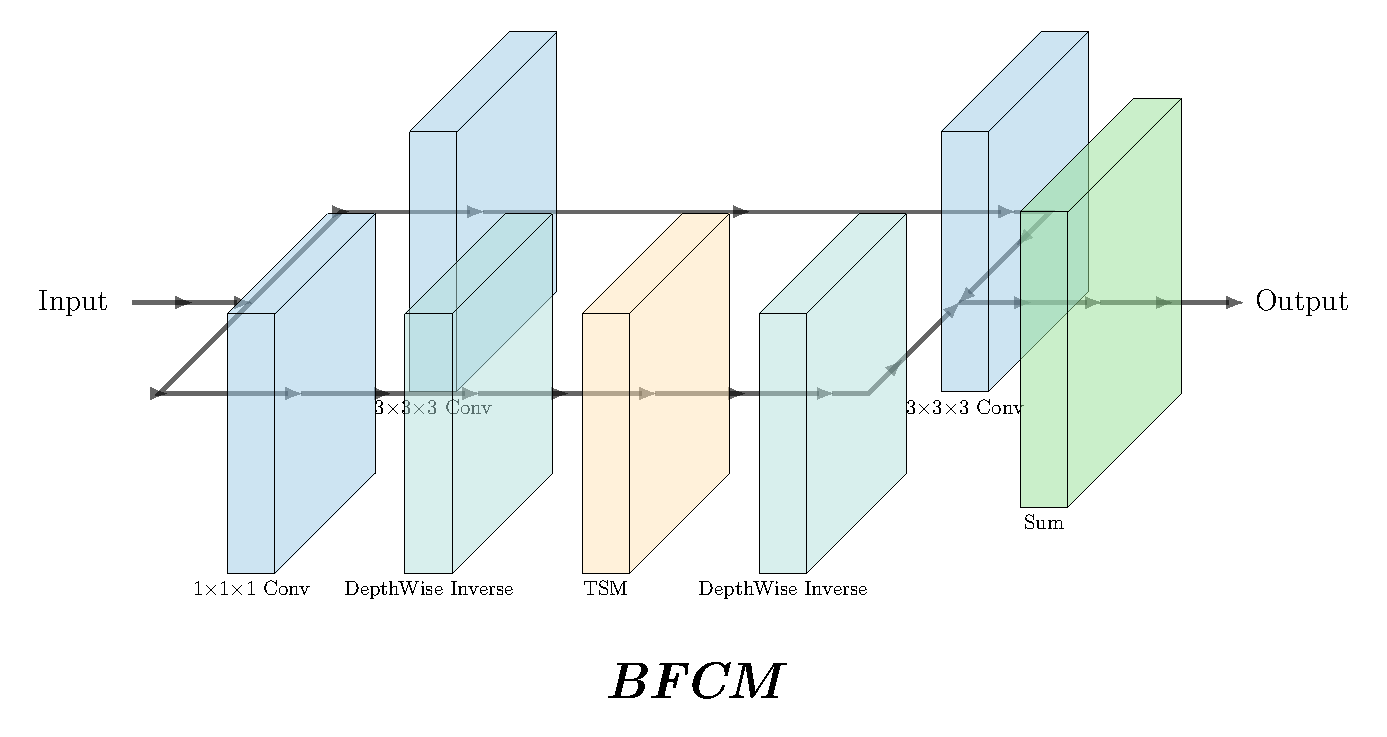
\includegraphics[
        width=16.5cm,  % <-- 设置第二个PDF的宽度
        page=1
    ]{modules/BFCM.pdf} % <-- 替换为你的第二个PDF文件名
};

%%%%%%%%%%%%%%%%%%%%%%%%%%%%%%%%%%%%%%%%%%%%%%%%%%%%%%%%%%%%%%%%%%%%%%%%%%%%%%%%%%%%%%%%
%% 8. 绘制图例 (Legend)
%%%%%%%%%%%%%%%%%%%%%%%%%%%%%%%%%%%%%%%%%%%%%%%%%%%%%%%%%%%%%%%%%%%%%%%%%%%%%%%%%%%%%%%%
\coordinate (legend_pos_1) at ($(pdf_anchor) + (-13.5cm, -11cm)$);
\coordinate (legend_pos_2) at ($(legend_pos_1) + (8cm, 0)$);
\coordinate (legend_pos_3) at ($(legend_pos_2) + (8cm, 0)$);
\coordinate (legend_pos_4) at ($(legend_pos_3) + (9.6cm, 0)$);

\pic at (legend_pos_1) {Box={
    name=lgd_pool, fill=\PoolColor, opacity=0.4, height=14, width=3, 
    depth=14, scale=0.2, caption={}, xlabel={{"",""}},
}};
\pic at (legend_pos_2) {Box={
    name=lgd_upsample, fill=\UnpoolColor, opacity=0.4, height=14, width=3, 
    depth=14, scale=0.2, caption={}, xlabel={{"",""}},
}};
\pic at (legend_pos_3) {Box={
    name=lgd_concat, fill=\CatColor, opacity=0.4, height=14, width=3, 
    depth=14, scale=0.2, caption={}, xlabel={{"",""}},
}};
\pic at (legend_pos_4) {Box={
    name=lgd_sigmoid, fill=\SoftmaxColor, opacity=0.4, height=14, width=3, 
    depth=14, scale=0.2, caption={}, xlabel={{"",""}},
}};

\node[anchor=west] at ($(lgd_pool-east) + (1.2cm, 0)$) {\Large\bfseries\itshape Pooling};
\node[anchor=west] at ($(lgd_upsample-east) + (1.2cm, 0)$) {\Large\bfseries\itshape Upsampling};
\node[anchor=west] at ($(lgd_concat-east) + (1cm, 0)$) {\Large\bfseries\itshape Channelwise  \ \ Concat};
\node(legend_text_4)[anchor=west] at ($(lgd_sigmoid-east) + (1cm, 0)$) {\Large\bfseries\itshape Sigmoid};

%%%%%%%%%%%%%%%%%%%%%%%%%%%%%%%%%%%%%%%%%%%%%%%%%%%%%%%%%%%%%%%%%%%%%%%%%%%%%%%%%%%%%%%%
%% 9. 绘制三个部分的边框
%%%%%%%%%%%%%%%%%%%%%%%%%%%%%%%%%%%%%%%%%%%%%%%%%%%%%%%%%%%%%%%%%%%%%%%%%%%%%%%%%%%%%%%%
\begin{scope}[on background layer]
\coordinate (top_anchor) at ($(img1)-(1cm,-3.5cm)$);
\coordinate (bottom_anchor) at ($(input_brace_label.south)-(0,18.5cm)$);
\node[framebox, fit=(top_anchor) (out_img3) (bottom_anchor), inner sep=20pt]{};

\coordinate (left_anchor) at ($(pdf_ffcm)-(6.25cm,-4cm)$);
\coordinate (right_anchor) at ($(pdf_bfcm)-(10cm,3.5cm)$);
\node[framebox, fit=(left_anchor) (right_anchor), inner sep=25pt]{};

\coordinate (left_anchor) at ($(pdf_ffcm)-(-9cm,-4cm)$);
\coordinate (right_anchor) at ($(pdf_bfcm)-(-7.3cm,3.5cm)$);
\node[framebox, fit=(left_anchor) (right_anchor), inner sep=25pt]{};

\coordinate (lgd_left_anchor) at ($(lgd_pool-west)-(1.8cm,-2.3cm)$);
\coordinate (lgd_right_anchor) at ($(legend_text_4)-(-1cm,2cm)$);
\node[framebox, fit=(lgd_left_anchor) (lgd_right_anchor), inner sep=15pt]{};
\end{scope} 

\end{tikzpicture}
\end{document}